
%        File: WeeklyResearchReport_4_19_21.tex
%     Created: Mon Apr 19 08:00 AM 2021 E
% Last Change: Mon Apr 19 08:00 AM 2021 E
%
\documentclass[a4paper]{article}
\usepackage{mathtools}
\usepackage{verbatim}
\usepackage{graphicx}
\usepackage{tabularx}
\usepackage{pgfplots}
\usepackage{adjustbox}
\usepackage{booktabs}
\makeatletter
\let\latex@xfloat=\@xfloat
\def\@xfloat #1[#2]{%
    \latex@xfloat #1[#2]%
    \def\baselinestretch{1}
    \@normalsize\normalsize
    \normalsize
}
\makeatother
\usepackage{amsmath}
\usepackage{mathtools}
\usepackage{epigraph}
\usepackage{cancel}
\usepackage{xcolor}
\newcommand\Ccancel[2][black]{\renewcommand\CancelColor{\color{#1}}\cancel{#2}}
\usepackage{algorithm}
\usepackage{graphicx}
\usepackage[noend]{algpseudocode}
\usepackage{gnuplot-lua-tikz}
\usepackage[utf8]{inputenc}
\usepackage{pgfplots}
\usepackage{tabularx}
\DeclareUnicodeCharacter{2212}{−}
\usepgfplotslibrary{groupplots,dateplot}
\usetikzlibrary{patterns,shapes.arrows}
\pgfplotsset{compat=newest}
\begin{document}
\begin{titlepage}

    \title{
    Daily Research Report}

    \author{ Jeffrey Severino \\
        University of Toledo \\
        Toledo, OH  43606 \\
    email: jseveri@rockets.utoledo.edu}


    \maketitle

\end{titlepage}
\section{Current Research Direction}
The goal is to complete the validation for SWIRL by creating a range of test
cases. The last step to complete each case is to include the pressure mode shape
as a function of axial wavenumber. The goal is to confirm that the corresponding 
mode shape for a given axial wavenumber resembles the modes produced 
from the eigensolver in SWIRL. 

\section{Research Performed}
The axial wavenumbers for a uniform flow case where $m = 2$ , $M = 0.3$ and 
$k = -1$ is presented. 

 \begin{figure}[h!]
     \centering
     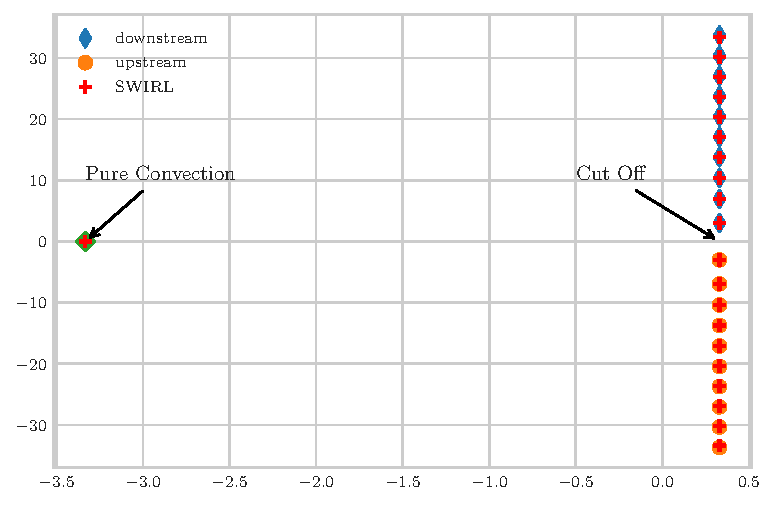
\includegraphics[width=\textwidth]{/home/jeff-severino/SWIRL/CodeRun/03-plotReport/tex-outputs/T1.pdf}
 \end{figure}

 The acoustic modes are along the cut off line (parallel to the imaginary axis)
 and the convective modes are to the left or right of the line. 

 The analytical mode shape is going to be 

 \begin{equation}
     p' = p(r) e^{i(m \theta + k_x x - \omega t)}
 \end{equation}
 If we only want to look at things with respect to $x$, let's set $\theta = 0$
 $t = 0$, $p(r) = 1 (?)$, then


 \begin{equation}
     p' = e^{\pm i k_x x }
 \end{equation}

 When plotting this I get the following:
 \begin{figure}[h!]
     \centering
     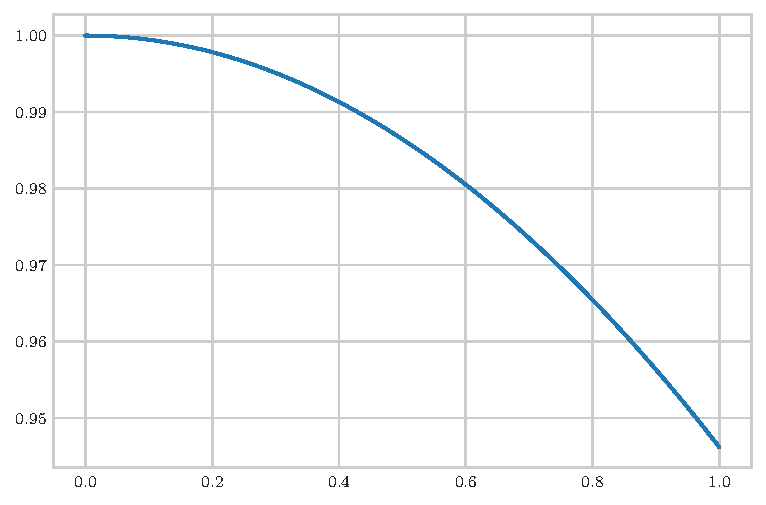
\includegraphics{k_x_0_re.pdf}
     \caption{Analytical Mode Shapes for $k_x,0$}
     \label{fig:kx0}
 \end{figure}

 \begin{figure}[h!]
     \centering
     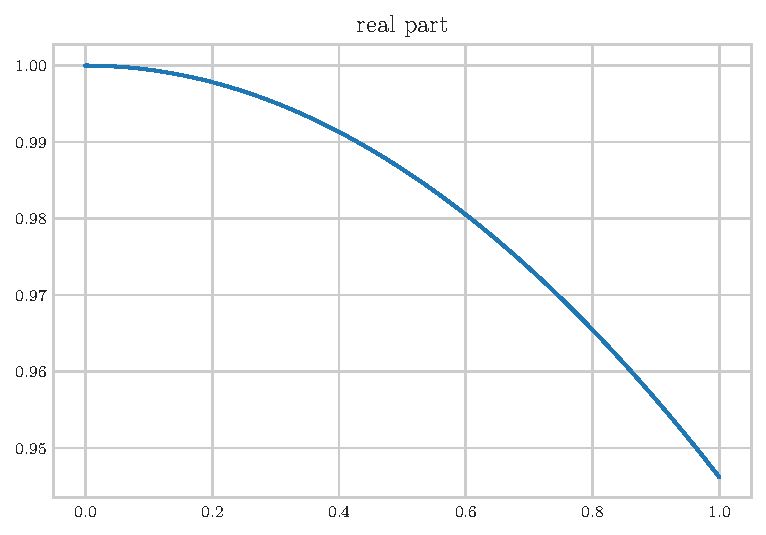
\includegraphics{k_x_1_re.pdf}
     \caption{Analytical Mode Shapes for $k_x,1$}
     \label{fig:kx0}
 \end{figure}

 \begin{figure}[h!]
     \centering
     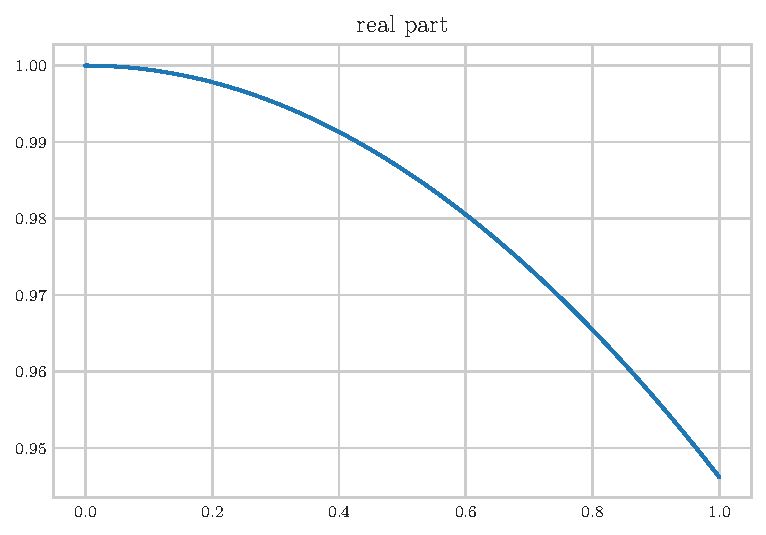
\includegraphics{k_x_2_re.pdf}
     \caption{Analytical Mode Shapes for $k_x,2$}
     \label{fig:kx0}
 \end{figure}

 \begin{figure}[h!]
     \centering
     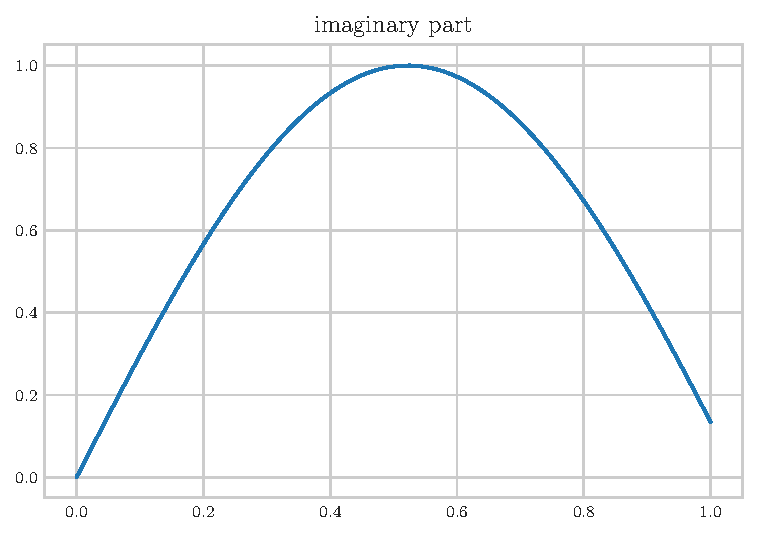
\includegraphics{k_x_0_im.pdf}
     \caption{Analytical Mode Shapes for $k_x,0$}
 \end{figure}
 \begin{figure}[h!]
     \centering
     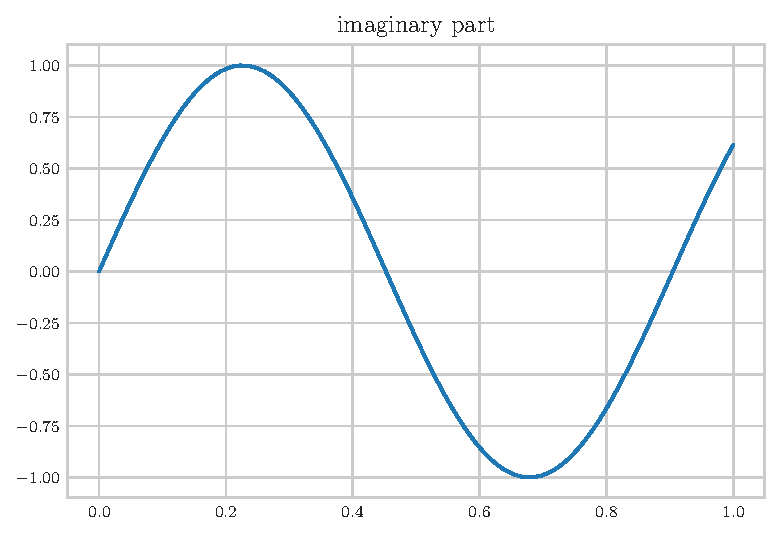
\includegraphics{k_x_1_im.pdf}
     \caption{Analytical Mode Shapes for $k_x,1$}
 \end{figure}
 \begin{figure}[h!]
     \centering
     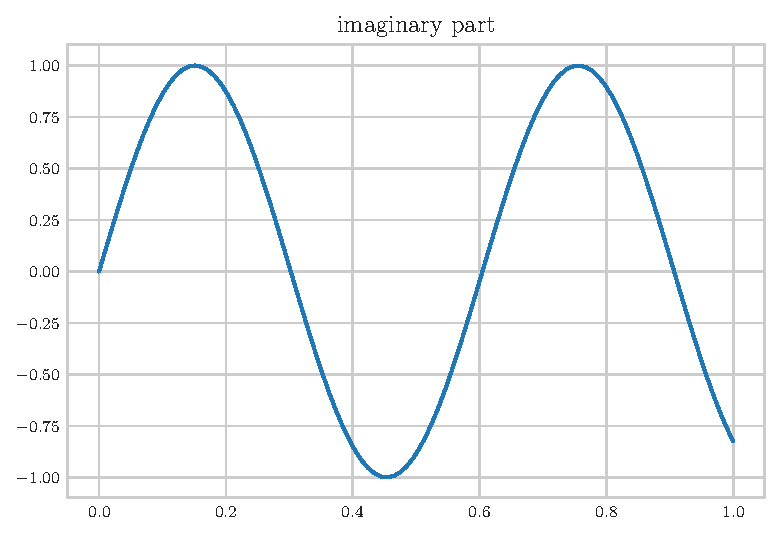
\includegraphics{k_x_2_im.pdf}
     \caption{Analytical Mode Shapes for $k_x,2$}
 \end{figure}
\begin{tiny}
 \begin{verbatim}
     \input{gam.nonconv.0128}
 \end{verbatim}
\end{tiny}
\section{Issues and concerns}
it is apparent that there is something off. I think I need to look at the plus and minus 
of $k_x$. Also, I have to be sure that my data types are consistent. The data type
conflict would be obvious in F90\dots The zero crossings in the imaginary part are off.
Figure 5 has 2 zero crossings besides the origin and Figure 6 has 3. The good thing
is that the number of zero crossings are increasing with axial wavenumber index
but I should be making hypotheses of what I expect to see and I thought I would 
see this behavior in the real part as well. 

\section{Planned Research}
\end{document}


